\section{Decisões Arquiteturais}\label{sec:decisoes}

Durante o decorrer do desenvolvimento do projeto foi necessário tomar diferentes decisões arquiteturais, tendo em conta não só o progresso do trabalho como também a fluidez do sistema.

No planeamento da arquitetura levada a cabo pelo grupo foi definido o uso das diferentes plataformas.
\\
\begin{itemize}
\item [\textbf{JADE}]
	\item Agente Mother
	\item Agente Estação
	\item Agente Manual
	\item Agente Utilizador
	\item Meteorologia
	\item Agente Decider
\\
\item [\textbf{JADEX}]
	\item Agente Utilizador
\\
\item [\textbf{JESS}]
	\item Agente Decider
\end{itemize}
\vspace{5mm}
Achamos também útil definir já os custos consoante as áreas que os utilizadores percorrem mediante o seu percurso previamente calculado.
Para isto definimos três patamares de preço:
\begin{description}
	\item [Estação com baixa afluência (\leq 25\%)] - 50\% do custo base
	\item [Estação com média afluência (26\% - 74\%)] - 100\% do custo base
	\item [Estação com alta afluência (\geq75\%)] - 150\% do custo base
\end{description}
\vspace{5mm}

Os utilizadores têm definido uma gama de parâmetros que, ao serem criados, assumem. Estes parâmetros são os seguintes:
\begin{itemize}
\item [\textbf{Estado de Espírito}]
	\item 1 - Depressivo
	\item 2 - Triste
	\item 3 - Neutro
	\item 4 - Contente
	\item 5 - Eufórico
	
\item [\textbf{Idade}]: Entre 12 anos e 80 anos.

\item [\textbf{Sexo}]
	\item 1 - Masculino
	\item 2 - Feminino

\newpage

\item [\textbf{Doenças}]
	\item 1 - Saudável
	\item 2 - Grande doença
	\item 3 - Pequena doença

\ \item [\textbf{Condição Física}]
	\item 1 - Pessoa Passiva
	\item 2 - Pessoa Pouco Ativa
	\item 3 - Pessoa Ativa
	\item 4 - Atleta
	\item 5 - Atleta Profissional
\end{itemize}
\vspace{5mm}
Assim e baseando-se nestes dados, o algoritmo que toma a decisão se um determinado utilizador deve ou não aceitar uma oferta de uma estação é baseado numa árvore em que os níveis da árvore são os parâmetros mais relevantes para o cálculo do próximo caso.
Existe um ficheiro com dados de cálculos anteriores que é usado para calcular uma percentagem de utilizadores que aceitaram ou rejeitaram determinada oferta consoante os parâmetros, esse valor é usado como "peso" e multiplicado pelos valores gerados pela "Mother" aquando da criança. Depois disso, se a estação que estiver mais perto for a mais barata vai diretamente para essa, se a mais barata for diferente da que está mais perto, faz o cálculo consoante os pesos, se esse resultado for menor que 10, vai para a mais perto, se for maior ou igual vai para a mais barata.

\begin{figure}[H]
    \centering
    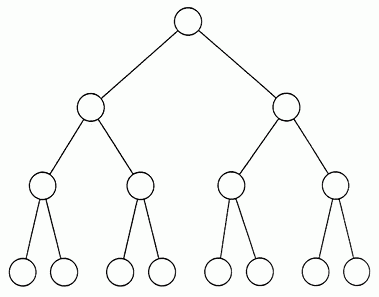
\includegraphics[scale=0.8]{bin.png}
    \caption{Árvore de Decisão}
    \label{fig:Arvore}
\end{figure}